\section{Flavour Physics}
%
We still need a theory of the quark masses (and mixing). The third generation in the standard model consists of:
\begin{itemize}
\item \textbf{$\tau$ lepton: } discovered in 1975 at SLAC, with a mass $m_\tau = $ 1.78 GeV. This was relatively unexpected;
\item \textbf{$b$ quark: } discovered in 1977 at Fermilab, with a mass $m_b$ = 5 GeV. Seen in the form of the $\Upsilon = b\bar{b}$ particle with mass 10 GeV;
\item \textbf{$\nu_\tau$ neutrino: } finally seen in 2000 at Fermilab. This was very difficult!;
\item \textbf{$t$ quark: } finally discovered in 1995 at the Tevatron, Fermilab, with a mass $m_t$ = 175 GeV.
\end{itemize}
The top quark is very heavy: $m_t > m_W, m_Z, m_h$, and decays very quickly via $t \to Wb$ before it can hadronise. Because of anomalies it does not decouple from low energy processes; its involvement is needed for consistency.

There are only three generations (3 light neutrinos).
%
\subsection{The Quark Masses}
%
As with leptons, these must arise through Yukawa interactions. We have left-handed doublets and right-handed singlets under SU(2)$_L$:
\[ Q_L^i = \left( \begin{array}{cc}
u_L   \\
d_L  \end{array} \right), \qquad
\left( \begin{array}{cc}
c_L   \\
s_L   \end{array} \right), \qquad
\left( \begin{array}{cc}
t_L   \\
b_L   \end{array} \right);\]
\[ 
u_R^i = \qquad u_R, \qquad c_R, \qquad t_R, \qquad;
\]
\[ 
d_R^i = \qquad d^\prime_R, \qquad s^\prime_R, \qquad b_R, \qquad \text{for } i=1,2,3.
\]
where the "up-type" quarks appear on the top row and "down-type" quarks on the bottom row. For leptons we introduced Yukawa coupling to a complex doublet
\[\phi = \left( \begin{array}{cc}
\phi^+ \\
\phi^0 \end{array} \right),
\]
which can give mass to the down-type quarks through $<\phi^0> = v$. What about up-type quarks? Consider the conjugate field
\[
\phi^c \equiv (i\sigma_2)\phi^+ = \left( \begin{array}{cc}
0 & 1   \\
-1 & 0  \end{array} \right) 
\left( \begin{array}{cc}
\phi^{+ *}   \\
\phi^{0 *}  \end{array} \right) = 
\left( \begin{array}{cc}
\phi^{0 *}   \\
-\phi^{+ *}  \end{array} \right).
\]
Clearly $\phi^c$ has $Y = - \frac{1}{2}$. Moreover
\begin{equation}
(i\sigma_2)\sigma_i^* = -\sigma_i(i\sigma_2),
\end{equation}
so under SU(2)$_L$, $\phi \to U \phi = \exp(\frac{i}{2}\underline{\alpha}\cdot \underline{\sigma})$, and
\begin{equation}
\phi^c \to (i\sigma_2)e^{-\frac{i}{2}\underline{\alpha}\cdot\underline{\sigma}^*} \phi^* = e^{+\frac{i}{2}\underline{\alpha}\cdot{\sigma}}(i\sigma_2)\phi^* = U \phi^c,
\end{equation}
so $\phi^c$ is also a doublet under SU(2)$_L$.

Note that this works because SU(2) is "pseudoreal". This implies also that $tr \sigma_i \{\sigma_j, \sigma_k \} = 0$, i.e. it is anomaly free. This does not generalise to SU(N), for N>2: for this we would need a second Higgs doublet. So besides $\bar{Q}_L\phi d_R$, which gives mass to down-type quarks, we also have $\bar{Q}_L\phi^c u_R$, which gives mass to up-type quarks. (What does the missing line here say?)

So the most general Yukawa term for quarks is
\begin{equation}
\mathcal{L}_{Y} = -(Y_{ij}^d \bar{Q}_L^i \phi d_R^j + h.c.) - (Y_{ij}^u \bar{Q}_L^i \phi^c u_R^j + h.c.),
\end{equation}
where $Y^u$, $Y^d$ are two arbitrary 3$\times$3 matrices. After spontaneous symmetry breaking
\begin{equation}
\phi \to \frac{v}{\sqrt{2}}\begin{pmatrix} 0 \\ 1 \end{pmatrix},
\qquad \phi^c \to \frac{v}{\sqrt{2}}\begin{pmatrix} 1 \\ 0 \end{pmatrix}.
\end{equation}
So defining mass matrices $M_{ij}^u = \frac{v}{\sqrt{2}}Y_{ij}^u$; $M_{ij}^d = \frac{v}{\sqrt{2}}Y_{ij}^d$, we have
\begin{equation}
\mathcal{L}_{Y} = -(M_{ij}^u \bar{u}_L^i u_R^j + h.c.) - (M_{ij}^d \bar{d}_L^i d_R^j + h.c.).
\end{equation}
Note that there is mixing between up-type quarks and between down-type quarks, but not between different types: this would violate U(1)$_Y$. We need to diagonalise the mass matrices, in order to find the "mass basis". Consider $M^u$: $M^{u \dagger} M^u$ is hermitian, so the real positive eigenvalues are $m_u^2$, $m_c^2$ and $m_t^2$. Similarly, $M^{d \dagger} M^d$ is hermitian, so the real positive eigenvalues are $m_d^2$, $m_s^2$ and $m_b^2$.
\subsubsection{Lemma: $\exists$ unitary matrices $L$ and $R$ such that $LMR^\dagger=D$, a diagonal matrix with masses $m_u^2$, $m_c^2$ and $m_t^2$ (or $m_d$, $m_s^2$ and $m_b^2$).}
\textbf{Proof: }
\begin{equation}
(M^\dagger M)^\dagger = M^\dagger M, 
\end{equation}
so $\exists$ a unitary matrix $R$ such that
\begin{equation}
R^\dagger(M^\dagger M)R = D^2,
\end{equation}
where $D$ is a diagonal matrix with real, positive eigenvalues. Then define $L = MRD^{-1}$, so
\begin{equation}
L^\dagger = D^{-1}R^\dagger M^\dagger, \qquad L^\dagger L = D^{-1}R^\dagger M^\dagger MR D^{-1} = 1,
\end{equation}
i.e. $L$ is unitary and $L^\dagger MR = D^{-1}R^\dagger M^\dagger MR = D$, so we have
\begin{equation}
L^{u \dagger}M^u R^u = D^u, \qquad L^{d \dagger}M^d R^d = D^d,
\end{equation}
and if we let
\begin{equation}
\begin{split}
u_R \to R^u u_R \qquad u_L \to L^u u_L \\
d_R \to R^d d_R \qquad d_L \to L^d d_L
\end{split}
\end{equation}
then the mass terms become diagonal:
\begin{equation}
- \sum_{q = u,c,t} m_q(\bar{q}_L q_R + \bar{q}_R q_L) - \sum_{q = d,s,b} m_q(\bar{q}_L q_R + \bar{q}_R q_L) = - \sum_{q=u,c,t,d,s,b} m_q \bar{q}{q}.
\end{equation}
It is easy to see that the kinetic term remains diagonal:
\begin{equation}
\mathcal{L}_{D,\ kin} = \sum_{q = d,s,b}(\bar{q}_L i \slashed{\partial} q_L + \bar{q}_R i \slashed{\partial} q_R),
\end{equation}
and $L^u$, $L^d$, $R^u$, $R^d$ are all hermitian. Likewise, the quark contribution to the neutral current
\begin{equation}
J_\mu^{NC} = \sum_{q=u,c,t}\bar{q}\gamma_\mu\bigg(\frac{-4}{3}\sin^2\theta_w +\frac{1}{2}(1-\gamma^5)\bigg)q + \sum_{q=d,s,b}\bar{q}\gamma_\mu\bigg(\frac{2}{3}\sin^2\theta_w -\frac{1}{2}(1-\gamma^5)\bigg)q,
\end{equation}
is invariant, since 
\begin{equation}
\bar{q}\gamma^\mu q = \bar{q}_L\gamma^\mu q_L + \bar{q}_L\gamma^\mu q_R.
\end{equation}
This is the GIM mechanism, which we saw earlier in the course.
%
\subsection{The CKM Matrix}
%
Charge conjugation relates up-type quarks to down-type quarks, so 
\begin{equation}
\begin{split}
\frac{1}{2} J_\mu^h = \sum_i \bar{u}_L^i \gamma_\mu d_L^i &\to \sum_{ijk} \bar{u}_L^i(L^{u \dagger})^{ij}\gamma_\mu(L^{d})^{jk}d_L^k \\
&\equiv \sum_{ij} \bar{u}_L^i \gamma_\mu V^{ij} d_L^j,
\end{split}
\end{equation}
where $V = L^{u \dagger} L^d$ is the CKM matrix, named after Cabibbo, Kobayashi and Maskawa (1973). The CKM matrix mixes the charged current interactions.

$V$ is unitary: $V^\dagger V = L^{d \dagger}L^u L^{u \dagger} L^d = 1$. There are $N$ generations, so $V$ is an $N\times N$ complex matrix and has $2N^2$ real parameters. Unitarity gives $N^2$ constraints, so there are $N^2$ remaining real parameters. However, phase changes of the form $u_L^i \to \exp(i\alpha_i)u_L^i$, $d_L^i \to \exp(i\beta_i)d_L^i$ can remove $ 2N-1$ of these parameters. So overall we have 
\begin{equation}
N^2 - (2N-1) = (N-1)^2 = \frac{N}{2}(N-1) + \frac{1}{2}(N-1)(N-2).
\end{equation}
An $N\times N$ real orthogonal matrix has $\frac{N}{2}(N-1)$ parameters, so we have $\frac{N}{2}(N-1)$ angles and $\frac{1}{2}(N-1)(N-2)$ phases. Consdering different numbers of generations:
\begin{enumerate}
\item $N=1$:

$V=1$ and there is no mixing.
\item $N=2$:

There is one angle and are no phases.
\begin{equation}
V = \begin{pmatrix}
\cos\theta_L & \sin\theta_L \\
-\sin\theta_L & \cos\theta_c
\end{pmatrix},
\end{equation}
where $\theta_c$ is the Cabbibo angle.
\item $N=3$:

There are three angles and one phase.
\begin{equation}
V = \begin{pmatrix}
V_{ud} & V_{us} & V_{ub} \\
V_{cd} & V_{cs} & V_{cb} \\
V_{td} & V_{ts} & V_{tb} 
\end{pmatrix} =
\begin{pmatrix}
1 & 0 & 0 \\
0 & c_1 & s_1 \\
0 & -s_1 & c_1 
\end{pmatrix}
\begin{pmatrix}
c_2 & 0 & s_2e^{i\delta} \\
0 & 1 & 0 \\
-s_2 e^{i\delta} & 0 & c_2
\end{pmatrix}
\begin{pmatrix}
c_3 & s_3 & 0 \\
-s_3 & c_3 & 0 \\
0 & 0 & 1
\end{pmatrix},
\end{equation}
where we have used the notation $c_i = \cos\theta_i$, $s_i = \sin\theta_i$, with $\theta_i$ being the Euler angles and $\delta$ being the phase.
\end{enumerate}
\textbf{Notes: }
\begin{itemize}
\item We can put the mixing into down-type quarks (as is convention) $d_L^{i \prime} = V^{* ij} d_L^j$ or into up-type quarks $\bar{u}_L^{j \prime} = \bar{u}_L^iV^{ij}$, and the physics is unchanged.
\item $V$ depends on only $L^u$ and $L^d$ (not $R^u$ and $R^d$), because charged current is left-handed.
\item For leptons, because up-type leptons (i.e. neutrinos) are massless, we can absorb $V$ into $\nu_L$ with impunity; there is no mixing. We see that mixing and mass are intimately related.
\item Mixing follows directly from spontaneous symmetry breaking for quark masses, but it's not pretty... we have 10 new parameters (6 masses, 3 angles and 1 phase).
\item The charged current Feynman rules pick up factors of elements of $V$ and $V^\dagger$, e.g.
\newline
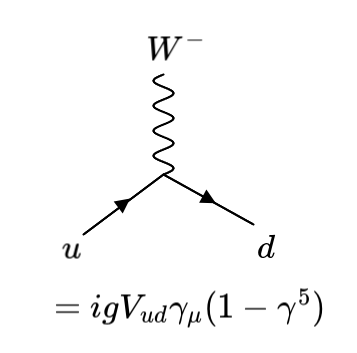
\includegraphics[width=0.4\linewidth]{figs/46a.png}
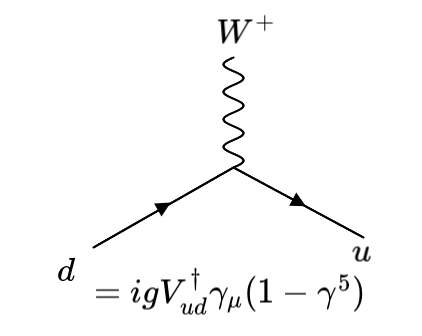
\includegraphics[width=0.4\linewidth]{figs/46b.png}
\end{itemize}
%
\subsection{Unitarity Triangles}
%
Testing for unitarity is equialent to testing for the condition $VV^\dagger =1$. There are different ways of doing this:
\begin{enumerate}
\item \textbf{Universality tests: }
There are three tests of the form $(V^\dagger V)_{ii}=1$, e.g.
$|V_{ud}|^2 +|V_{us}|^2 +|V_{ub}|^2 = 1$.
\item \textbf{Triangle tests: }
There are six tests of the form $(V^\dagger V)_{ij}=0$ for $i \neq j$, e.g.
$V^*_{ub}V_{ud} + V^*_{cb}V_{cd} + V^*_{tb}V_{td} = 0$. 

This is a triangle because it is a sum of three complex numbers. The diagram on the right shows the different connections between the quark types.
\newline
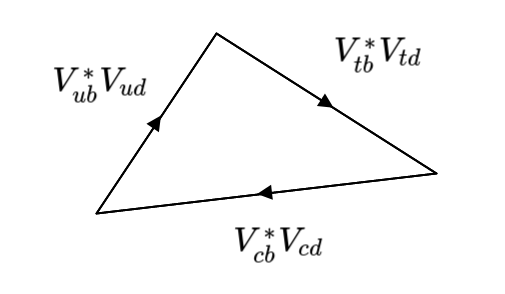
\includegraphics[width=0.6\linewidth]{figs/47a.png}
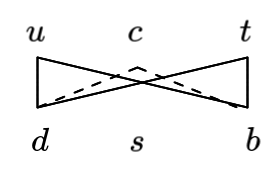
\includegraphics[width=0.3\linewidth]{figs/47b.png}
\end{enumerate}
\textbf{Determining $|V_{ij}|$: }
\begin{itemize}
\item The top left part of $V$ (which doesn't involve $t$ or $b$ quarks) is determined by measuring $\theta_c$ as above. More specifically: $|V_{ud}|$ is determined through $\beta$ and pion decay, $|V_{us}|$ through kaon and tau decays, and $|V_{cd}|$ and $|V_{cs}|$ are determined through $D$ semileptonic decays such as $D \to \pi l \nu$ and $D \to K l \nu$.
\item Additional elements involving the $b$ quark but not the $t$ quark (i.e. "B physics") are determined by $B$ semileptonic decays such as $B \to \pi l \nu$ and $B \to D l \nu$. 
\item $|V_{tb}|$ is determined through single top producgion $t \to bW$, but $|V_{ts}|$ and $|V_{td}|$ are very hard to measure directly. We can use corrections to loop calculations to find these (see later).
\end{itemize}
The results of the combined fits are usefully summarised by the Wolfenstein parametrisation (1983):
\begin{equation}
V = \begin{pmatrix}
1-\frac{\lambda^2}{2} & \lambda & A\lambda^3(\rho - i\eta) \\
-\lambda &  1-\frac{\lambda^2}{2} & A \lambda^2\\
A\lambda^3(1-\rho-i\eta) & -A\lambda^2 & 1 
\end{pmatrix} + \mathcal{O}(\lambda^4),
\end{equation}
where $\lambda \approx \sin\theta_c \approx\ 0.225$, $A \approx\ 0.8$, $\rho \approx\ 0.12$ and $\eta \approx 0.36$ are $\mathcal{O}(1)$. Since $\lambda \gg \lambda^2 \gg \lambda^3$, this expresses a curious hierarchy of the off-diagonal elements, which is not understood! 

Considering the various universality tests and triangles, we can see that in this parametrisation $V$ is unitary.

